\section{Creare un progetto con JavaFx}
    Ora che avete tutto pronto, è im momento di creare un progetto con JavaFx, per farlo useremo Gradle, uno dei due build tool disponibili per Java.
    
    \subsection{Gradle}
        Un build tool è uno strumento che automatizza il processo di compilazione del codice sorgente, gestione delle dipendenze, esecuzione dei 
        test e creazione dei pacchetti eseguibili o distribuzioni del software. Una delle caratteristiche principali di Gradle è la 
        gestione delle dipendenze, che permette di dichiarare le dipendenze del progetto in modo semplice e le scarica automaticamente dai repository, 
        come pip per python o npm per node. Noi lo utilizzeremo proprio per gestire JavaFx, così da non dover scaricare a mano la libreria e la documentazione
        e cosa più importante non dovremo configurare a mano i moduli di JavaFx quando eseguiremo il progetto.

    \subsection{Nuovo progetto}
    Aprite IntelliJ e cliccate sul tasto \textbf{New Project}, come tipo di progetto scegliete Java, dategli il nome che preferite e salvatelo in una cartella a 
    vostra scelta.
    \begin{warningbox}
        Non scegliete come percorso per il progetto una chiavetta usb, sono memorie lente e questo renderebbe l'ide praticamente inutilizzabile.
        Imparate invece ad usare git.
    \end{warningbox}
    Importante è selezionare come \textbf{Build system Gradle}, e come \textbf{Gradle DSL Groovy}.Togliete pure la spunta su Add sample code.
    \begin{figure}[H]
        \centering
        \graphicspath{{src/capitoli/05/img/}}
        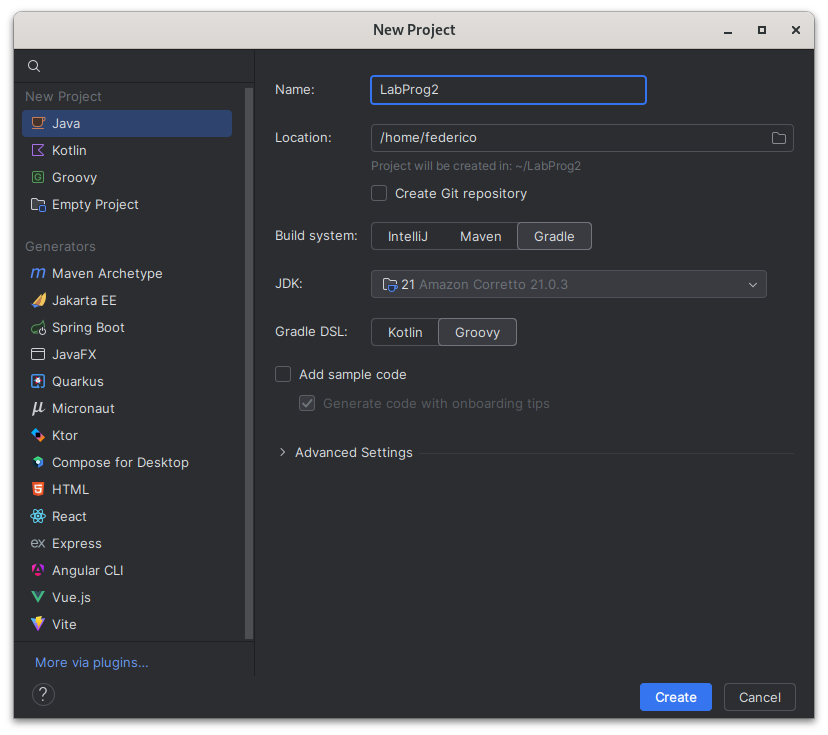
\includegraphics[width=\textwidth]{new_project.png}
        \caption{Creazione di un nuovo progetto con Gradle}
        \label{fig:Creazione di un nuovo progetto con Gradle}
    \end{figure}
    cliccate infine su Create e attendente la fine del processo.

    \subsection{Il file build.gradle}
    Una volta che il progetto sarà stato creato, vi si aprirà il file \textbf{build.gradle}, qui si specifica, tra le altre cose le dipendenze, 
    e come eseguire il vostro progetto. Se non vi si dovesse aprire in automatico, basta cercare il file nella barra laterale. Cancellate il 
    contenuto e incollate questo:
    \needspace{17\baselineskip}
    \begin{ret}
        \begin{lstlisting}[language=Groovy]
plugins {
    id 'application'
    id 'org.openjfx.javafxplugin' version '0.1.0'
}

group = 'org.example'
version = '1.0-SNAPSHOT'

repositories {
    mavenCentral()
}

javafx {
    version = "22" // versione di JavaFx
    modules = [ 'javafx.controls' ]
}

mainClassName = "Main"
        \end{lstlisting}
    \end{ret}
    \begin{warningbox}
        Controllate sul sito di \href{JavaFx}{https://gluonhq.com/products/javafx/} l'ultima versione compatibile con di JavaFx con il vostro jdk.
    \end{warningbox}
    \begin{figure}[H]
        \centering
        \graphicspath{{src/capitoli/05/img/}}
        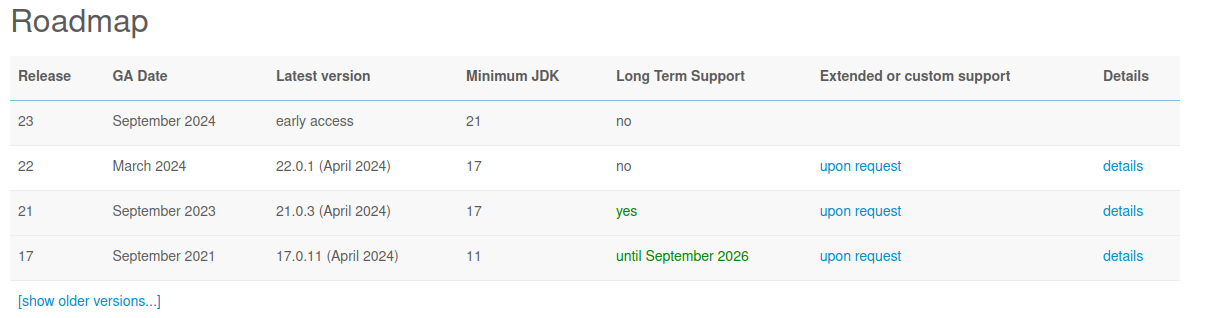
\includegraphics[width=\textwidth]{javafx_versions.png}
        \caption{Tabella con le versioni di JavaFx}
        \label{fig:Tabella con le versioni di JavaFx}
    \end{figure}    

    \subsection{Run configurations}
        Adesso che avete configurato Gradle per utilizzare JavaFx, cliccate in alto a destra il menù \textbf{Current File$\rightarrow$Edit Configurations$\rightarrow$+$\rightarrow$Gradle}
        \begin{figure}[H]
            \centering
            \graphicspath{{src/capitoli/05/img/}}
            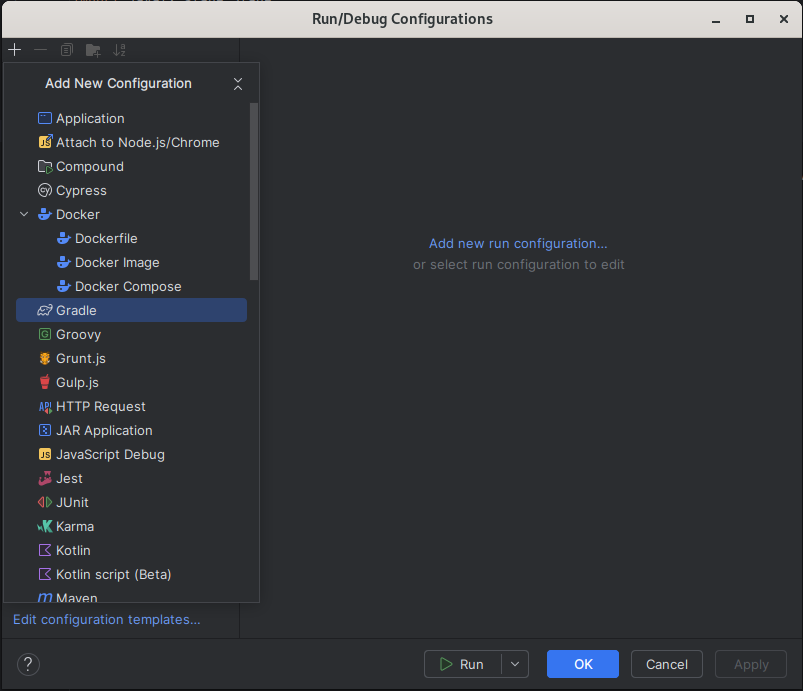
\includegraphics[width=\textwidth]{new_run_config.png}
            \caption{Menù opzioni di run}
            \label{fig:Menù opzioni di run}
        \end{figure}
        sotto \textbf{Run} nel campo di testo inserite il comando \texttt{run} questo specificherà che quando cliccherete il tasto esegui (quello a forma di 
        rettangolo verde) o il tasto di debug (quello a forma di insetto verde) eseguirà il comando run di Gradle caricando il modulo di JavaFx.
        L'opzione di run dovrebbe essere come questa:
        \begin{figure}[H]
            \centering
            \graphicspath{{src/capitoli/05/img/}}
            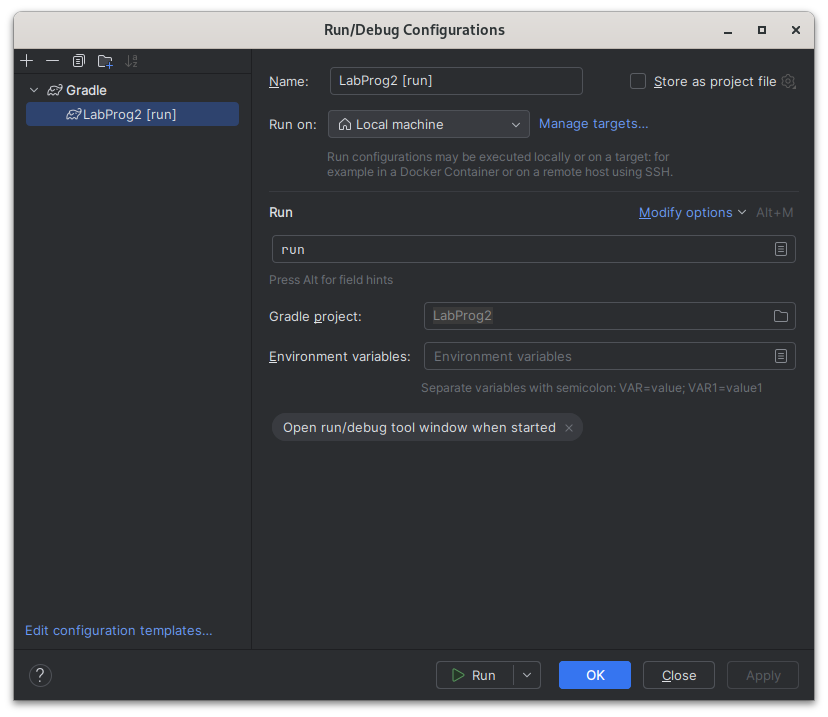
\includegraphics[width=\textwidth]{run_config.png}
            \caption{Opzione di run corretta per JavaFx}
            \label{fig:Opzione di run corretta per JavaFx}
        \end{figure}
    
    \subsection{Main di test}
        A questo punto per verificare che tutto sia correttamente configurato, aprite la cartella src, cancellate pure la sotto-cartella test e dentro la 
        sotto-cartella java create una nuova classe java chiamata Main. Cancellate tutto ciò che IntelliJ vi avrà creato e incollateci questo:
        \needspace{21\baselineskip}
        \begin{lstlisting}[language=Java]
import javafx.application.Application;
import javafx.scene.Scene;
import javafx.scene.control.Label;
import javafx.scene.layout.StackPane;
import javafx.stage.Stage;

public class Main extends Application {

    @Override
    public void start(Stage stage) {
        String javafxVersion = System.getProperty("javafx.version");
        Label l = new Label("Hello, JavaFX " + javafxVersion);
        Scene scene = new Scene(new StackPane(l), 640, 480);
        stage.setScene(scene);
        stage.show();
    }

    public static void main(String[] args) {
        launch();
    }
}            
        \end{lstlisting}
        Se tutto è configurato correttamente, cliccando il tasto di Run dovreste vedere una finestra come questa, con la versione di JavaFx che avete 
        specificato precedentemente.
        \begin{figure}[H]
            \centering
            \graphicspath{{src/capitoli/05/img/}}
            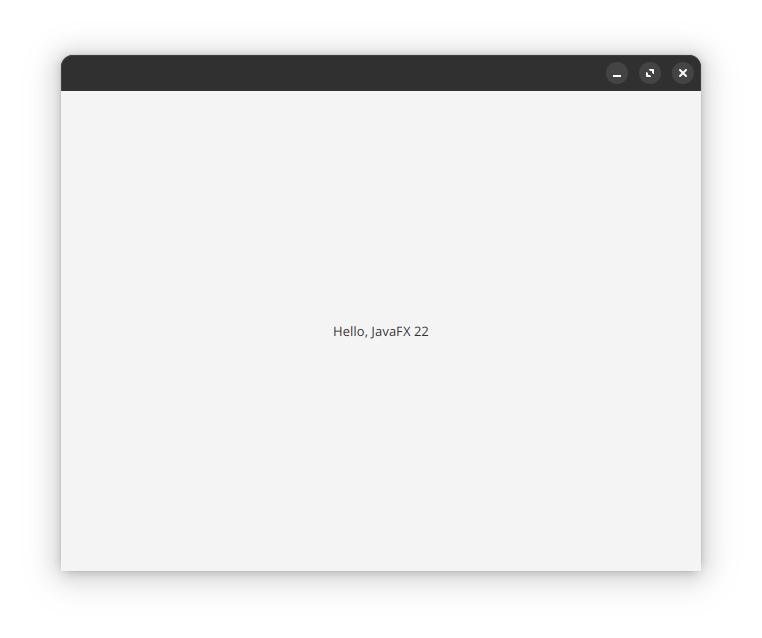
\includegraphics[width=\textwidth]{javafx_running.png}
            \caption{Finestra di prova}
            \label{fig:Finestra di prova}
        \end{figure}
        Non vi resta che seguire i vari laboratori, utilizzando la classe main che avete creato come base per completare le esercitazioni.